\documentclass[final]{beamer} % beamer 3.10: do NOT use option hyperref={pdfpagelabels=false} !
% Copyright (c) 2025 Dominik Szajerman <dominik.szajerman@p.lodz.pl> Karolina Nowak <karolina.nowak@p.lodz.pl>
\mode<presentation>{\usetheme{Berlin}}
\beamertemplatenavigationsymbolsempty
%
\usepackage[english]{babel}
\usepackage[T1]{fontenc}
\usepackage[utf8]{inputenc}
\usepackage{amsmath,amsthm,amssymb,latexsym}
\usefonttheme[onlymath]{serif}
\boldmath
\usepackage[orientation=portrait,size=custom,width=70.7,height=100.0,scale=1.45]
{beamerposter}%custom=b1%,grid,debug
\setbeamersize{text margin left=1.5cm,text margin right=1.5cm} 

\usepackage{graphicx}
\usepackage{subcaption}
\usepackage[super]{nth}
\usepackage{lipsum}

\setbeamertemplate{headline}{%
        \vspace{1.5cm}%
        \hspace{1.5cm}%
        
\includegraphics[height=6.1cm]{figures/logo-pl-institute.png}\hfill%
        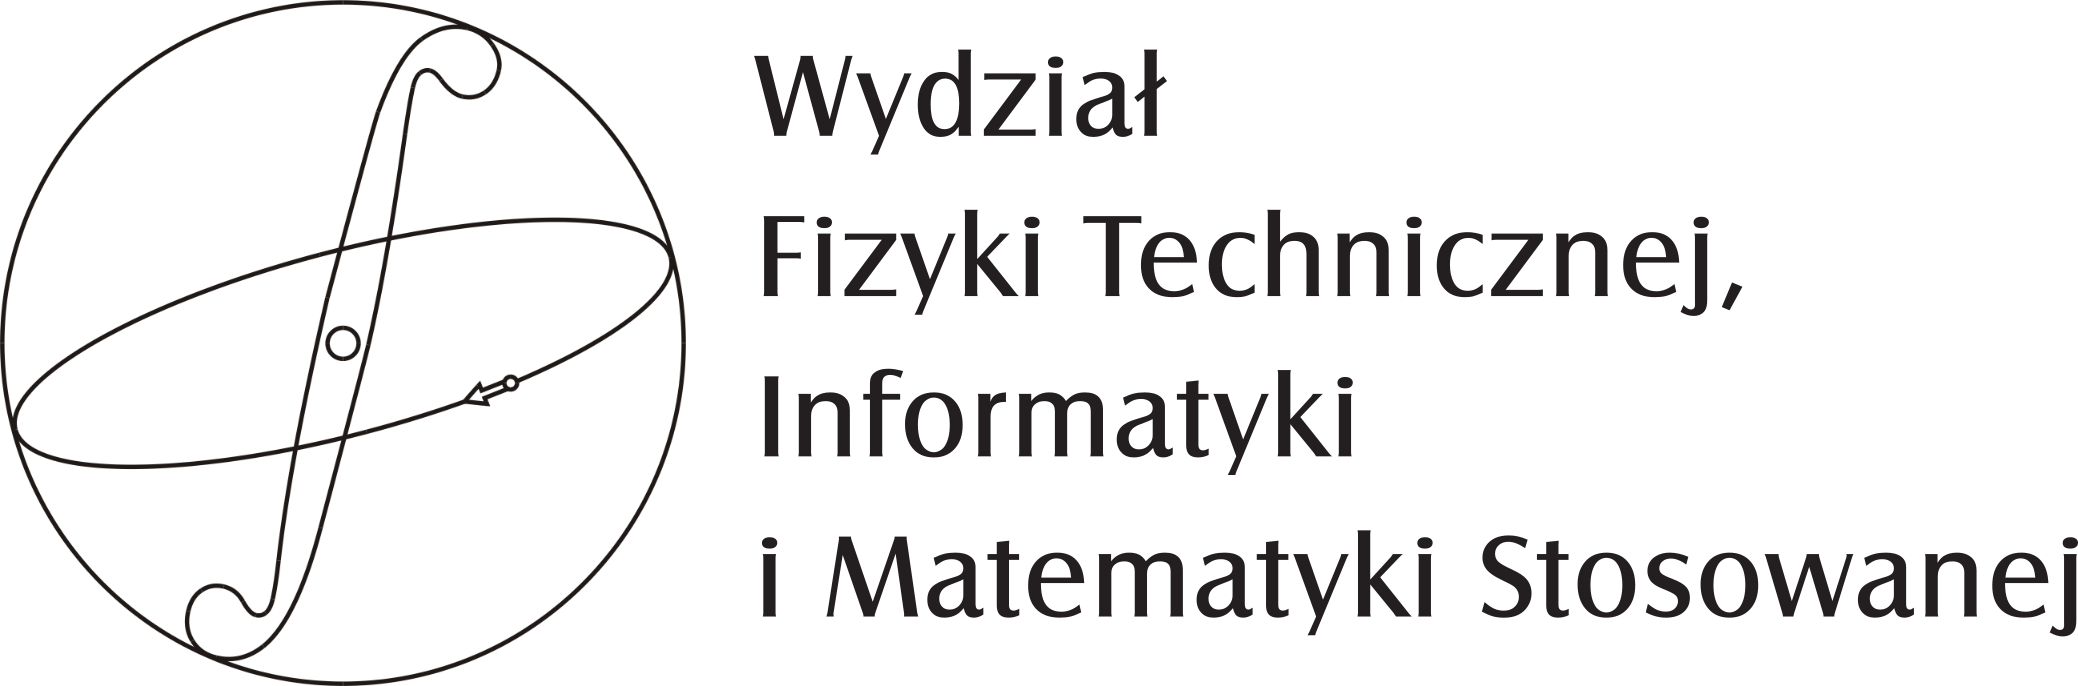
\includegraphics[height=4.7cm]{figures/logo-ftims.png}\hfill%
        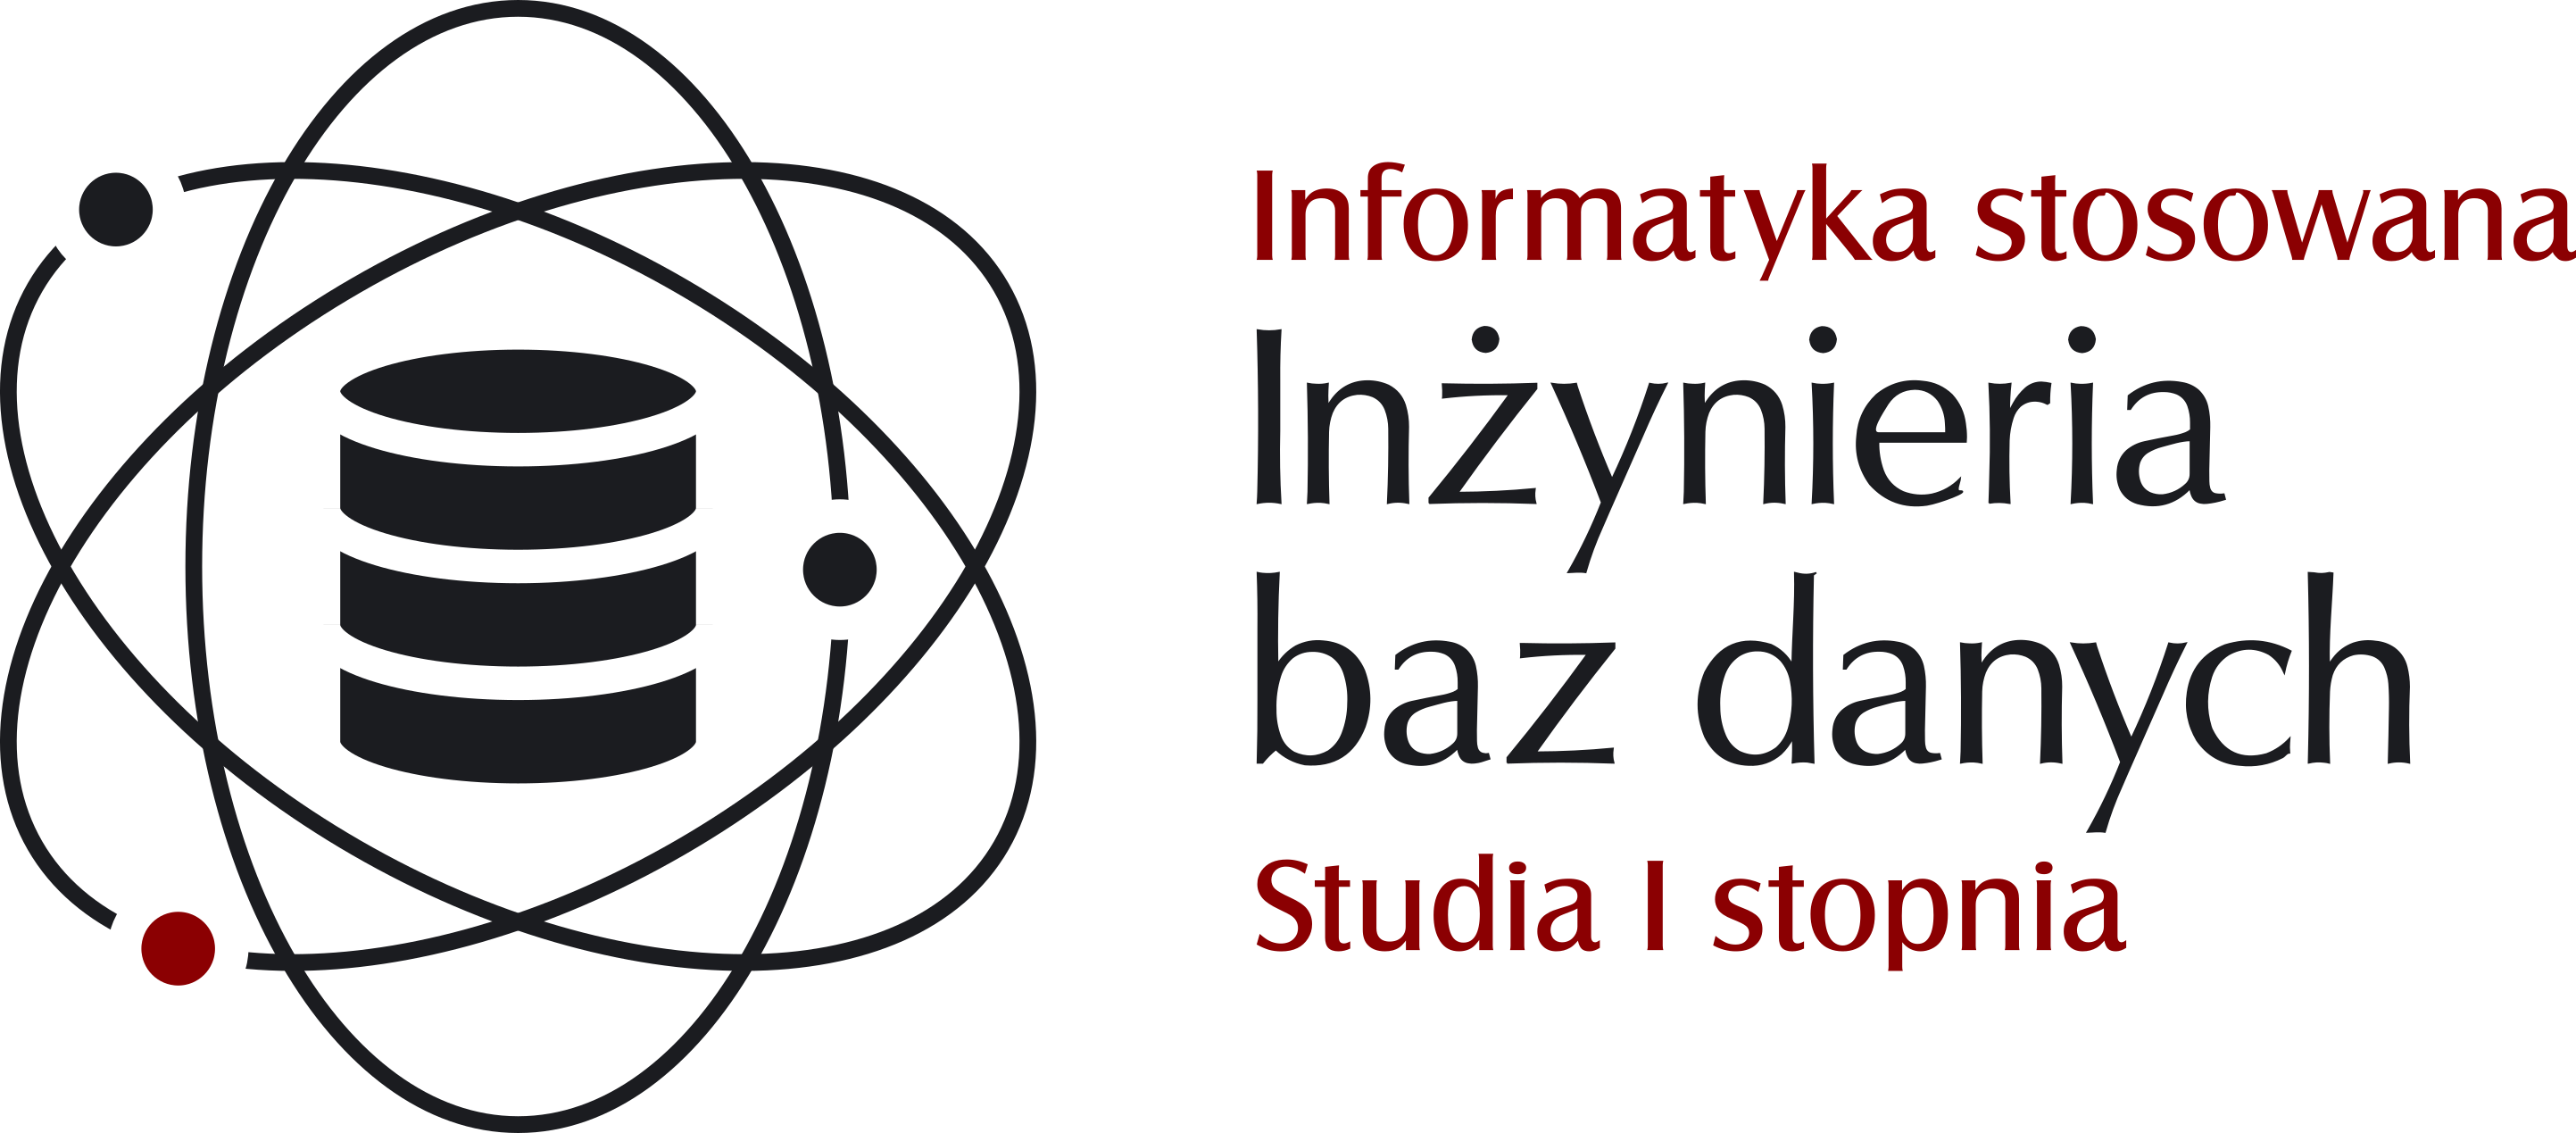
\includegraphics[height=5.3cm]{figures/logo-ibd.png}\hfill%
        
\includegraphics[height=4.2cm]{figures/HRK logo.png}%
        \hspace{1.5cm}
 }

\addtobeamertemplate{footline}{}{\vskip1.75cm}

\definecolor{PLcolor}{rgb}{0.475, 0.102, 0.125}
\usecolortheme[named=PLcolor]{structure}

\title[\hspace{1cm} HRK CRM]{HRK CRM -- System Zarządzania Klientami i Umowami}
\author[\hspace{1cm} Zespół AlfaTeam67]{Zespół AlfaTeam67}
\institute[Instytut Informatyki, Politechnika Łódzka, al. Politechniki 8, 93-590 Łódź \hspace{1cm}]{Instytut Informatyki, Politechnika Łódzka}
\date{Czerwiec 2026}

\graphicspath{ {figures/} }

\begin{document}

\renewcommand{\abstractname}{Streszczenie}
\renewcommand{\figurename}{Rysunek}
\renewcommand{\tablename}{Tabela}

\begin{frame}{}
\maketitle
%\vfill
\begin{abstract}
\centering
System HRK CRM to innowacyjne rozwiązanie klasy CRM zrealizowane dla firmy HRK Payroll Consulting. Jego nadrzędnym celem jest cyfryzacja procesów związanych z zarządzaniem bazą klientów oraz rozległą dokumentacją umów. Platforma automatyzuje rutynowy cykl życia kontraktów, proces waloryzacji oraz raportowanie wskaźników KPI. Wyróżnikiem jest wbudowany asystent sztucznej inteligencji, pomagający analizować dokumenty z zachowaniem pełnej poufności danych firmowych.
\end{abstract}
\begin{columns}[T]
\begin{column}[T]{0.48\textwidth}

\begin{block}{Wstęp}

W obliczu rosnącej liczby kontraktów, standardowe arkusze kalkulacyjne stają się niewystarczające. System HRK CRM powstał, aby rozwiązać problem rozproszonych danych i ręcznych wyliczeń.

Główne moduły aplikacji obejmują:
\begin{itemize}
    \item \textbf{Zarządzanie Umowami:} Kompleksowa baza kontrahentów pozwalająca na śledzenie historii współpracy i organizację dokumentów.
    \item \textbf{Proces Waloryzacji:} Moduł automatyzujący wyliczanie nowych stawek w oparciu o aktualne wskaźniki (np. inflacyjne).
    \item \textbf{Inteligentne Alerty i KPI:} Powiadomienia o terminach wygaśnięcia umów oraz analityczny dashboard do oceny rentowności projektów.
\end{itemize}
Dostęp do platformy zapewnia mechanizm logowania jednokrotnego (Active Directory SSO).
\end{block}

\begin{block}{Projekt aplikacji}

Zastosowano wydajną architekturę klient-serwer opartą na bezstanowym REST API. Całość uruchamiana jest z wykorzystaniem konteneryzacji \textbf{Docker}, co znacząco ułatwia zarządzanie aplikacją, replikację środowisk oraz jej bezproblemową migrację. Podział na izolowane serwisy gwarantuje dużą elastyczność i odporność na błędy. Wykorzystanie otwartych standardów zapewnia łatwość przyszłego utrzymania kodu i onboardingu nowych programistów. Wdrożono również mechanizmy stałego monitorowania kondycji kontenerów. Dzięki temu cała architektura jest przygotowana na płynne skalowanie horyzontalne w przyszłości.

\begin{itemize}
\item \textbf{Interfejs Użytkownika:} Dynamiczna aplikacja webowa zbudowana w \textbf{React 19} (z językiem TypeScript). Wykorzystano doceniany i spójny framework \textbf{Tailwind CSS}. Za zarządzanie stanem i optymalne ładowanie danych odpowiadają wyspecjalizowane biblioteki do asynchronicznego cachowania zapytań HTTP.
\item \textbf{Logika Serwera:} Niezwykle wydajne API napisane w \textbf{Pythonie 3.12} przy wsparciu asynchronicznego frameworka \textbf{FastAPI} oraz dojrzałego ORM \textbf{SQLAlchemy}. Kod zaplecza przechodzi rygorystyczne testy automatyczne oraz statyczną analizę bezpieczeństwa.
\item \textbf{Składowanie Danych:} Dojrzała relacyjna baza danych \textbf{PostgreSQL} rozszerzona o \texttt{pgvector} dla potrzeb AI. Szybkie repozytorium tysięcy plików i skanów umów PDF zrealizowano przez wdrożenie lokalnej usługi \textbf{MinIO}, stanowiącej bezpieczną alternatywę dla rozwiązań chmurowych.
\end{itemize}

\end{block}

\end{column}

\begin{column}[T]{0.48\textwidth}

\begin{block}{Implementacja}

Najbardziej innowacyjnym elementem systemu jest wbudowany moduł doradczy – "Advisor". Ze względu na poufność danych zrezygnowano z zewnętrznego AI na rzecz w pełni lokalnego modelu językowego \textbf{phi-3.5} (\textbf{Ollama}).

System wykorzystuje architekturę \textbf{Retrieval-Augmented Generation (RAG)}:
\begin{enumerate}
    \item \textbf{Parsowanie:} Umowy PDF są dzielone na mniejsze paragrafy (chunks) i poddawane wektoryzacji.
    \item \textbf{Składowanie Wektorów:} Reprezentacje liczbowe (embeddings) trafiają bezpośrednio do bazy PostgreSQL (rozszerzenie \texttt{pgvector}).
    \item \textbf{Wyszukiwanie:} Zapytania doradców HR używają wyszukiwania semantycznego do wydobycia najbardziej relewantnych klauzul.
    \item \textbf{Odpowiedź Modelu:} Precyzyjny fragment kontraktu pozwala LLM wygenerować jasną i udokumentowaną odpowiedź.
\end{enumerate}

\begin{figure}[h]
\centering
\begin{subfigure}{0.49\textwidth}
    \includegraphics[width=\textwidth]{example-image}
\end{subfigure}
\hfill
\begin{subfigure}{0.49\textwidth}
    \includegraphics[width=\textwidth]{example-image}
\end{subfigure}
\caption{Przepływ danych w modelu AI oraz widok interakcji.}
\label{fig:arch_ui}
\end{figure}

Taka implementacja redukuje czas wielogodzinnej, ręcznej weryfikacji dokumentów do sekund.

\end{block}

\begin{block}{Podsumowanie}

HRK CRM łączy wymogi bezpiecznego oprogramowania biznesowego z innowacjami sztucznej inteligencji. Platforma nie tylko eliminuje monotonne procesy manualne i przyspiesza obrót dokumentami, ale też rewolucjonizuje samą pracę z tekstem prawnym poprzez asystenta RAG. Wykorzystanie sprawdzonych technologii otwiera drogę do dalszej rozbudowy o moduły analityczne i łatwe integrowanie w przyszłości.

\end{block}

\begin{block}{Podziękowania}

Serdecznie dziękujemy firmie HRK Payroll Consulting za cenną współpracę i możliwość realizacji projektu. Wyrazy wdzięczności kierujemy również do prowadzących przedmiot Zespołowy Projekt Programistyczny za wsparcie merytoryczne.

\end{block}

\end{column}
\end{columns}
    \vfill
\end{frame}
\end{document}